% Seccion consolidada del TFM sobre el pico real de mma.sync. Incluir con % Seccion consolidada del TFM sobre el pico real de mma.sync. Incluir con % Seccion consolidada del TFM sobre el pico real de mma.sync. Incluir con % Seccion consolidada del TFM sobre el pico real de mma.sync. Incluir con \input{docs/TFM/pico_mma.tex}.
% Requiere: \usepackage{graphicx,booktabs}. Ajusta rutas si compilas desde otro dir.
% Datos: results/hennessy/run_pico_mma/ultimo (job 20834) y matmul con reloj (jobs 20835--20837).
% GB10 (sm_121, 48 SMs), CUDA 13.0.

\section{Pico real de los tensor cores: microbenchmark de \texttt{mma.sync}}
\label{sec:pico-mma}

En Blackwell GeForce (sm\_120/sm\_121) no existen \texttt{wgmma} ni \texttt{tcgen05}, y todos
los DSLs acaban emitiendo \texttt{mma.sync} (§~\ref{sec:tma}). El techo de los kernels es, por
tanto, el ritmo de esa instrucción. NVIDIA no lo publica para sm\_121 y las cifras de catálogo
mezclan \emph{sparsity} y precisiones bajas, así que hasta ahora los kernels solo podían
compararse entre sí o con cuBLAS. Esta sección mide ese techo directamente, instrucción a
instrucción, y expresa los resultados del TFM como porcentaje del pico alcanzable.

\subsection{Método}

Un kernel CUDA con PTX en línea (\texttt{src/Microbench/pico\_mma\_ext.cu}) en el que cada warp
carga una sola vez sus fragmentos A y B en registros (datos aleatorios del tipo
correspondiente, no ceros, para no falsear la potencia). Después encadena
$\mathit{iters}\times\mathit{ILP}$ instrucciones \texttt{mma.sync} sobre ILP acumuladores
independientes, \textbf{sin ningún acceso a memoria}, y al final escribe un único valor por hilo
para que el compilador no elimine el bucle. Se lanza un bloque por SM y se barren los warps por
SM (1, 4, 8, 16, 32) y el ILP (1, 2, 4, 8). La medida es la mediana de \texttt{do\_bench}, y en
paralelo se muestrean el reloj SM y la potencia por NVML, de lo que se obtiene la cifra
intrínseca de la arquitectura: FLOP/ciclo/SM.

Cada instrucción se compila para \texttt{sm\_121a}, la variante específica de la arquitectura
y la única que acepta las MMA con escalado por bloques. Con \texttt{-arch=sm\_121a -shared},
nvcc genera PTX para \texttt{compute\_121} sin la \texttt{a} y ptxas las rechaza; hace falta
\texttt{-gencode=arch=compute\_121a,code=sm\_121a} explícito. El SASS (\texttt{cuobjdump})
confirma que todas se ejecutan como instrucciones de tensor core.

\subsection{Resultados}

\begin{figure}[htbp]
  \centering
  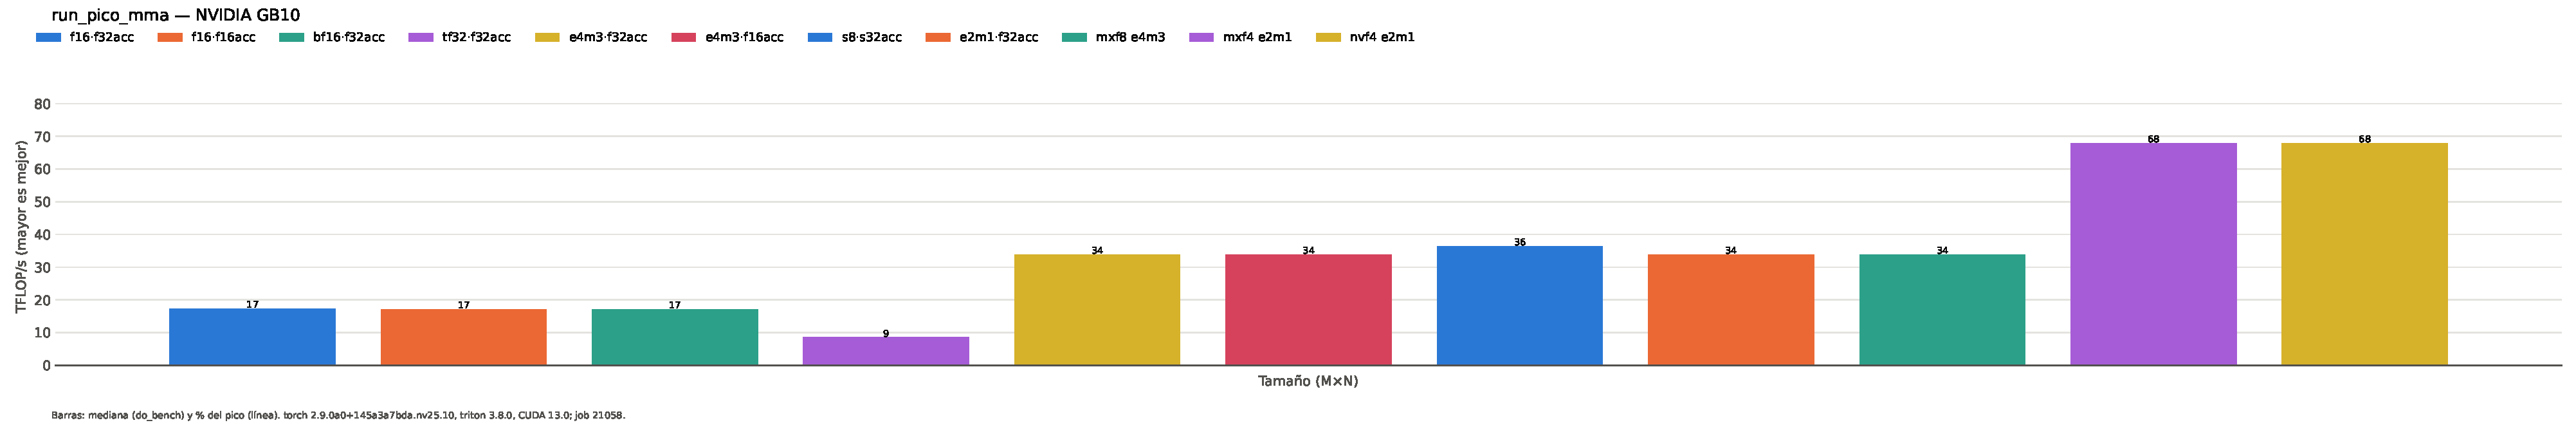
\includegraphics[width=\linewidth]{resultados/hennessy/figuras/run_pico_mma.pdf}
  \caption{GB10: (a) pico medido por instrucción \texttt{mma.sync}; (b) saturación de la
  unidad MMA (f16$\to$f32) en función de los warps por SM y de los acumuladores
  independientes por warp (ILP).}
  \label{fig:pico-mma}
\end{figure}

\begin{table}[htbp]
  \centering\small
  \begin{tabular}{llrrr}
    \toprule
    instrucción PTX & SASS & pico (TFLOP/s) & FLOP/ciclo/SM & rel.\ a f16 \\
    \midrule
    \texttt{m16n8k8} tf32$\to$f32 & \texttt{HMMA.1688.F32.TF32} & 61{,}4 & 511 & 0{,}5$\times$ \\
    \texttt{m16n8k16} f16$\to$f32 & \texttt{HMMA.16816.F32} & \textbf{122{,}7} & 1\,024 & 1$\times$ \\
    \texttt{m16n8k16} f16$\to$f16 & \texttt{HMMA.16816.F16} & 122{,}8 & 1\,020 & 1$\times$ \\
    \texttt{m16n8k16} bf16$\to$f32 & \texttt{HMMA.16816.F32.BF16} & 122{,}8 & 1\,019 & 1$\times$ \\
    \texttt{m16n8k32} e4m3$\to$f32 & \texttt{QMMA.16832.F32.E4M3} & \textbf{243{,}3} & 2\,041 & 2$\times$ \\
    \texttt{m16n8k32} e4m3$\to$f16 & \texttt{QMMA.16832.F16.E4M3} & 243{,}5 & 2\,038 & 2$\times$ \\
    \texttt{m16n8k32} s8$\to$s32 & \texttt{IMMA.16832.S8.S8} & 243{,}9\,(TOP/s) & 2\,031 & 2$\times$ \\
    \texttt{kind::f8f6f4} e2m1 & \texttt{QMMA.16832.F32.E2M1} & 245{,}7 & 2\,051 & 2$\times$ \\
    \texttt{kind::mxf8f6f4} MXFP8 & \texttt{QMMA.SF.16832.E4M3.E8} & 242{,}9 & 2\,038 & 2$\times$ \\
    \texttt{kind::mxf4nvf4} MXFP4 & \texttt{OMMA.SF.16864.E2M1.E8} & \textbf{487{,}3} & 4\,089 & 4$\times$ \\
    \texttt{kind::mxf4nvf4} NVFP4 & \texttt{OMMA.SF.16864.E2M1.UE4M3} & 486{,}9 & 4\,085 & 4$\times$ \\
    \bottomrule
  \end{tabular}
  \caption{Pico de \texttt{mma.sync} en GB10 (job 20834), en ráfaga ($\sim$0{,}35~s por punto,
  reloj 2\,480--2\,520~MHz). En régimen sostenido la MMA pura mantiene 2\,424~MHz: 118{,}7 (f16) y
  237{,}3 (e4m3) TFLOP/s (job 20848). Barrido completo en \texttt{resultados/hennessy/run\_pico\_mma}.}
  \label{tab:pico-mma}
\end{table}

\subsection{Análisis del microbenchmark}

\begin{enumerate}
  \item \textbf{La unidad MMA hace 1\,024~FLOP/ciclo/SM en FP16} (512 FMA, 128 por subpartición):
  122{,}7~TFLOP/s en ráfaga ($48~\text{SMs}\times 2{,}5~\text{GHz}$) y 118{,}7 sostenidos
  (2{,}42~GHz). La cifra por ciclo es la intrínseca; los TFLOP/s dependen del reloj sostenido.
  \item \textbf{Acumular en FP16 no aporta nada}: f16$\to$f16 rinde igual que f16$\to$f32 (lo
  mismo con e4m3). A diferencia de las GeForce Ampere/Ada, GB10 no reduce a la mitad la
  acumulación en FP32.
  \item \textbf{La escalera de precisiones es limpia}: TF32 0{,}5$\times$, FP16/BF16 1$\times$,
  FP8/INT8 2$\times$, FP4 4$\times$. Pero el 4$\times$ de FP4 solo se obtiene con la instrucción
  \emph{block-scaled} \texttt{mxf4nvf4} (\texttt{OMMA}, $k=64$, FP4 empaquetado). El FP4 de
  \texttt{kind::f8f6f4} usa contenedores de 8~bits y rinde como FP8. El escalado por bloques
  (MXFP8, MXFP4, NVFP4) no tiene coste.
  \item \textbf{Saturar la MMA exige $\geq 8$ warps por SM} ($\geq 2$ por subpartición). La
  latencia de una MMA es de $\sim$28 ciclos, y un mismo warp no emite más de una cada
  $\sim$17 ciclos, mientras que la unidad acepta una cada 16 por subpartición. Con 4~warps/SM el
  máximo es el $\sim$94\,\%, sea cual sea el ILP (figura~\ref{fig:pico-mma}b).
\end{enumerate}

\subsection{Medir reloj y potencia en GB10}

Como el pico es $1\,024~\text{FLOP/ciclo/SM}\times 48\times\text{reloj}$, comparar un kernel con él
exige saber a qué reloj iba. En GB10 eso no es trivial (sondas, jobs 20844 y 20845). NVML solo
actualiza reloj y potencia cada $\sim$0{,}5~s, y la potencia de \texttt{nvmlDeviceGetPowerUsage}
es un promedio retrasado $\sim$1~s: al empezar una carga, la potencia instantánea
(\texttt{NVML\_FI\_DEV\_POWER\_INSTANT}) ya marca 100~W y la promedio aún 20~W. Además, bajo un
GEMM continuo el reloj tarda $\sim$0{,}5~s en bajar de 2\,410 a 2\,180~MHz. Una medida de
\texttt{do\_bench} ($\sim$0{,}6~s) cae, por tanto, sobre el transitorio. Por eso se mide en
\textbf{régimen sostenido} (\texttt{run\_sostenido}): 6~s seguidos tras 3~s de reposo, contando
solo los últimos 4~s y con potencia instantánea. Una lectura previa con potencia promedio
(``TMA ahorra un tercio de potencia'') resultó ser un artefacto de la medida.

\subsection{Los kernels del TFM frente al pico}

\begin{table}[htbp]
  \centering\small
  \begin{tabular}{lrrrrr}
    \toprule
    kernel ($8192^3$) & TFLOP/s & reloj (MHz) & potencia (W) & \% al mismo reloj & \% nominal \\
    \midrule
    \texttt{mma.sync} f16 (micro) & 118{,}7 & 2\,424 & 100 & 99{,}6 & 97 \\
    \texttt{mma.sync} e4m3 (micro) & 237{,}3 & 2\,424 & 99 & 99{,}6 & 98 \\
    cuBLAS fp16 & 94{,}4 & 2\,138 & 90 & \textbf{89{,}8} & 77 \\
    Triton fp16 & 90{,}6 & 2\,177 & 90 & 84{,}6 & 74 \\
    Triton + TMA fp16 & 93{,}8 & 2\,080 & 89 & \textbf{91{,}7} & 76 \\
    cuBLASLt FP8 & 182{,}9 & 2\,145 & 91 & 86{,}7 & 75 \\
    Triton FP8 & 144{,}0 & 2\,158 & 91 & 67{,}9 & 59 \\
    \bottomrule
  \end{tabular}
  \caption{Régimen sostenido en GB10 (job 20848). ``Al mismo reloj'': frente a
  $1\,024$ (fp16) o $2\,048$ (fp8)~FLOP/ciclo/SM $\times$ 48 SMs al reloj medido durante el
  kernel. ``Nominal'': frente a 122{,}7 / 243{,}3~TFLOP/s (ráfaga a $\sim$2{,}5~GHz).}
  \label{tab:pico-kernels}
\end{table}

\begin{figure}[htbp]
  \centering
  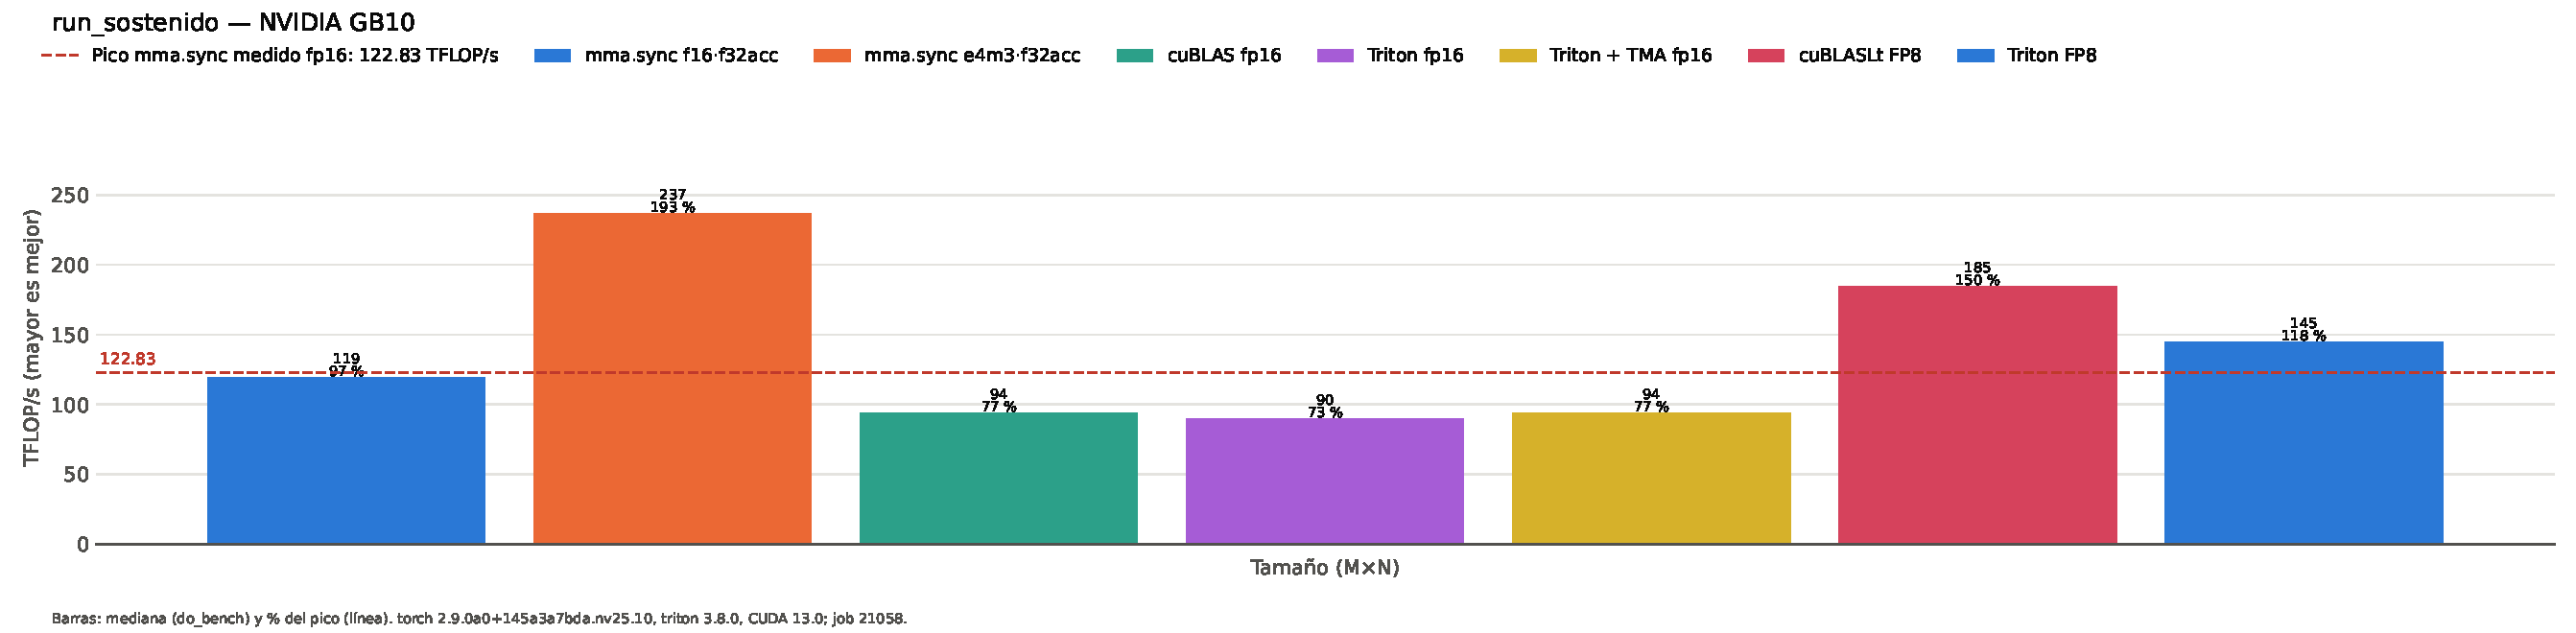
\includegraphics[width=\linewidth]{resultados/hennessy/figuras/run_sostenido.pdf}
  \caption{Régimen sostenido en GB10 (job 20848): (a) eficiencia por ciclo, como \% del pico de
  \texttt{mma.sync} al reloj de cada kernel; (b) reloj SM sostenido y potencia de GPU. La línea
  discontinua es el reloj que sostiene la MMA pura.}
  \label{fig:sostenido}
\end{figure}

En FlashAttention (jobs anteriores, sin reloj) los porcentajes sobre el pico nominal son: Triton
75\,\%, CuTe 74\,\% (normal y causal), SDPA 69\,\% y Helion 54\,\% (34\,\% causal, que además
no se salta el triángulo superior).

\begin{enumerate}
  \item \textbf{Ningún kernel real pasa del $\sim$77\,\% del pico nominal}, y el hueco tiene dos
  partes de tamaño parecido.
  \item \textbf{Reloj ($\sim$12--15 puntos).} La MMA pura sostiene 2\,424~MHz, pero cualquier
  GEMM real baja a 2\,080--2\,180~MHz, y lo hace con \emph{menos} potencia de GPU según NVML
  ($\sim$90 frente a 100~W). El límite no es, por tanto, la potencia de la GPU tal como la mide
  NVML. Una hipótesis plausible, pendiente de verificar, es el presupuesto total del chip, que
  comparte potencia y memoria con la CPU.
  \item \textbf{Por ciclo ($\sim$8--15 puntos).} A su propio reloj, cuBLAS y Triton + TMA llegan
  al 90--92\,\%. Lo que falta se pierde en alimentar \texttt{mma.sync} (\texttt{ldmatrix}, esperas
  de copia, sincronización, \emph{epilogue}).
  \item \textbf{TMA mejora la eficiencia por ciclo} (91{,}7 frente a 84{,}6\,\%), aunque su kernel
  sostiene un reloj algo menor. El neto es $+3{,}5\,\%$ (§~\ref{sec:tma}).
  \item \textbf{En FP8, Triton se queda en el 68\,\% a su reloj} (cuBLASLt, 87\,\%): hueco de
  \emph{scheduling} (§~\ref{sec:fp8}).
\end{enumerate}

\subsection{Conclusión}

La unidad MMA de GB10 hace \textbf{1\,024~FLOP/ciclo/SM en FP16/BF16, 2\,048 en FP8/INT8 y
4\,096 en MXFP4/NVFP4}, sin penalización por acumular en FP32 ni por el escalado por bloques: en
ráfaga, 122{,}7 / 243 / 487~TFLOP/s, y en régimen sostenido la MMA pura mantiene 2{,}42~GHz.
Saturarla requiere al menos dos warps por subpartición. Los mejores kernels del TFM sostienen el
75--77\,\% del pico nominal. Aproximadamente la mitad del hueco es reloj, porque un GEMM real
hace bajar GB10 a $\sim$2{,}1--2{,}2~GHz; la otra mitad se pierde por ciclo, alimentando la MMA.
A su propio reloj, estos kernels rinden el 87--92\,\% del pico. FP4 con escalado por bloques
duplica el techo de FP8 y es la palanca que queda por explotar.
.
% Requiere: \usepackage{graphicx,booktabs}. Ajusta rutas si compilas desde otro dir.
% Datos: results/hennessy/run_pico_mma/ultimo (job 20834) y matmul con reloj (jobs 20835--20837).
% GB10 (sm_121, 48 SMs), CUDA 13.0.

\section{Pico real de los tensor cores: microbenchmark de \texttt{mma.sync}}
\label{sec:pico-mma}

En Blackwell GeForce (sm\_120/sm\_121) no existen \texttt{wgmma} ni \texttt{tcgen05}, y todos
los DSLs acaban emitiendo \texttt{mma.sync} (§~\ref{sec:tma}). El techo de los kernels es, por
tanto, el ritmo de esa instrucción. NVIDIA no lo publica para sm\_121 y las cifras de catálogo
mezclan \emph{sparsity} y precisiones bajas, así que hasta ahora los kernels solo podían
compararse entre sí o con cuBLAS. Esta sección mide ese techo directamente, instrucción a
instrucción, y expresa los resultados del TFM como porcentaje del pico alcanzable.

\subsection{Método}

Un kernel CUDA con PTX en línea (\texttt{src/Microbench/pico\_mma\_ext.cu}) en el que cada warp
carga una sola vez sus fragmentos A y B en registros (datos aleatorios del tipo
correspondiente, no ceros, para no falsear la potencia). Después encadena
$\mathit{iters}\times\mathit{ILP}$ instrucciones \texttt{mma.sync} sobre ILP acumuladores
independientes, \textbf{sin ningún acceso a memoria}, y al final escribe un único valor por hilo
para que el compilador no elimine el bucle. Se lanza un bloque por SM y se barren los warps por
SM (1, 4, 8, 16, 32) y el ILP (1, 2, 4, 8). La medida es la mediana de \texttt{do\_bench}, y en
paralelo se muestrean el reloj SM y la potencia por NVML, de lo que se obtiene la cifra
intrínseca de la arquitectura: FLOP/ciclo/SM.

Cada instrucción se compila para \texttt{sm\_121a}, la variante específica de la arquitectura
y la única que acepta las MMA con escalado por bloques. Con \texttt{-arch=sm\_121a -shared},
nvcc genera PTX para \texttt{compute\_121} sin la \texttt{a} y ptxas las rechaza; hace falta
\texttt{-gencode=arch=compute\_121a,code=sm\_121a} explícito. El SASS (\texttt{cuobjdump})
confirma que todas se ejecutan como instrucciones de tensor core.

\subsection{Resultados}

\begin{figure}[htbp]
  \centering
  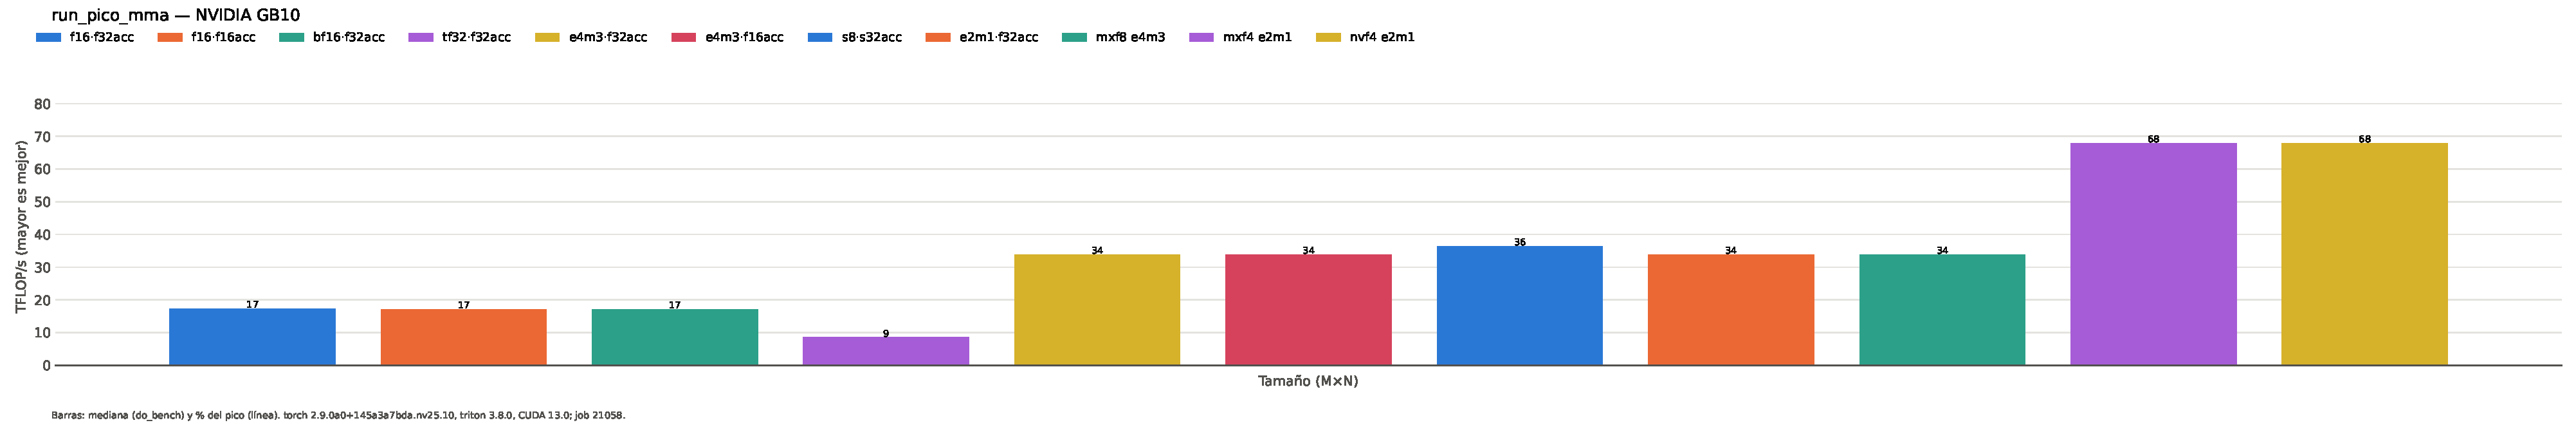
\includegraphics[width=\linewidth]{resultados/hennessy/figuras/run_pico_mma.pdf}
  \caption{GB10: (a) pico medido por instrucción \texttt{mma.sync}; (b) saturación de la
  unidad MMA (f16$\to$f32) en función de los warps por SM y de los acumuladores
  independientes por warp (ILP).}
  \label{fig:pico-mma}
\end{figure}

\begin{table}[htbp]
  \centering\small
  \begin{tabular}{llrrr}
    \toprule
    instrucción PTX & SASS & pico (TFLOP/s) & FLOP/ciclo/SM & rel.\ a f16 \\
    \midrule
    \texttt{m16n8k8} tf32$\to$f32 & \texttt{HMMA.1688.F32.TF32} & 61{,}4 & 511 & 0{,}5$\times$ \\
    \texttt{m16n8k16} f16$\to$f32 & \texttt{HMMA.16816.F32} & \textbf{122{,}7} & 1\,024 & 1$\times$ \\
    \texttt{m16n8k16} f16$\to$f16 & \texttt{HMMA.16816.F16} & 122{,}8 & 1\,020 & 1$\times$ \\
    \texttt{m16n8k16} bf16$\to$f32 & \texttt{HMMA.16816.F32.BF16} & 122{,}8 & 1\,019 & 1$\times$ \\
    \texttt{m16n8k32} e4m3$\to$f32 & \texttt{QMMA.16832.F32.E4M3} & \textbf{243{,}3} & 2\,041 & 2$\times$ \\
    \texttt{m16n8k32} e4m3$\to$f16 & \texttt{QMMA.16832.F16.E4M3} & 243{,}5 & 2\,038 & 2$\times$ \\
    \texttt{m16n8k32} s8$\to$s32 & \texttt{IMMA.16832.S8.S8} & 243{,}9\,(TOP/s) & 2\,031 & 2$\times$ \\
    \texttt{kind::f8f6f4} e2m1 & \texttt{QMMA.16832.F32.E2M1} & 245{,}7 & 2\,051 & 2$\times$ \\
    \texttt{kind::mxf8f6f4} MXFP8 & \texttt{QMMA.SF.16832.E4M3.E8} & 242{,}9 & 2\,038 & 2$\times$ \\
    \texttt{kind::mxf4nvf4} MXFP4 & \texttt{OMMA.SF.16864.E2M1.E8} & \textbf{487{,}3} & 4\,089 & 4$\times$ \\
    \texttt{kind::mxf4nvf4} NVFP4 & \texttt{OMMA.SF.16864.E2M1.UE4M3} & 486{,}9 & 4\,085 & 4$\times$ \\
    \bottomrule
  \end{tabular}
  \caption{Pico de \texttt{mma.sync} en GB10 (job 20834), en ráfaga ($\sim$0{,}35~s por punto,
  reloj 2\,480--2\,520~MHz). En régimen sostenido la MMA pura mantiene 2\,424~MHz: 118{,}7 (f16) y
  237{,}3 (e4m3) TFLOP/s (job 20848). Barrido completo en \texttt{resultados/hennessy/run\_pico\_mma}.}
  \label{tab:pico-mma}
\end{table}

\subsection{Análisis del microbenchmark}

\begin{enumerate}
  \item \textbf{La unidad MMA hace 1\,024~FLOP/ciclo/SM en FP16} (512 FMA, 128 por subpartición):
  122{,}7~TFLOP/s en ráfaga ($48~\text{SMs}\times 2{,}5~\text{GHz}$) y 118{,}7 sostenidos
  (2{,}42~GHz). La cifra por ciclo es la intrínseca; los TFLOP/s dependen del reloj sostenido.
  \item \textbf{Acumular en FP16 no aporta nada}: f16$\to$f16 rinde igual que f16$\to$f32 (lo
  mismo con e4m3). A diferencia de las GeForce Ampere/Ada, GB10 no reduce a la mitad la
  acumulación en FP32.
  \item \textbf{La escalera de precisiones es limpia}: TF32 0{,}5$\times$, FP16/BF16 1$\times$,
  FP8/INT8 2$\times$, FP4 4$\times$. Pero el 4$\times$ de FP4 solo se obtiene con la instrucción
  \emph{block-scaled} \texttt{mxf4nvf4} (\texttt{OMMA}, $k=64$, FP4 empaquetado). El FP4 de
  \texttt{kind::f8f6f4} usa contenedores de 8~bits y rinde como FP8. El escalado por bloques
  (MXFP8, MXFP4, NVFP4) no tiene coste.
  \item \textbf{Saturar la MMA exige $\geq 8$ warps por SM} ($\geq 2$ por subpartición). La
  latencia de una MMA es de $\sim$28 ciclos, y un mismo warp no emite más de una cada
  $\sim$17 ciclos, mientras que la unidad acepta una cada 16 por subpartición. Con 4~warps/SM el
  máximo es el $\sim$94\,\%, sea cual sea el ILP (figura~\ref{fig:pico-mma}b).
\end{enumerate}

\subsection{Medir reloj y potencia en GB10}

Como el pico es $1\,024~\text{FLOP/ciclo/SM}\times 48\times\text{reloj}$, comparar un kernel con él
exige saber a qué reloj iba. En GB10 eso no es trivial (sondas, jobs 20844 y 20845). NVML solo
actualiza reloj y potencia cada $\sim$0{,}5~s, y la potencia de \texttt{nvmlDeviceGetPowerUsage}
es un promedio retrasado $\sim$1~s: al empezar una carga, la potencia instantánea
(\texttt{NVML\_FI\_DEV\_POWER\_INSTANT}) ya marca 100~W y la promedio aún 20~W. Además, bajo un
GEMM continuo el reloj tarda $\sim$0{,}5~s en bajar de 2\,410 a 2\,180~MHz. Una medida de
\texttt{do\_bench} ($\sim$0{,}6~s) cae, por tanto, sobre el transitorio. Por eso se mide en
\textbf{régimen sostenido} (\texttt{run\_sostenido}): 6~s seguidos tras 3~s de reposo, contando
solo los últimos 4~s y con potencia instantánea. Una lectura previa con potencia promedio
(``TMA ahorra un tercio de potencia'') resultó ser un artefacto de la medida.

\subsection{Los kernels del TFM frente al pico}

\begin{table}[htbp]
  \centering\small
  \begin{tabular}{lrrrrr}
    \toprule
    kernel ($8192^3$) & TFLOP/s & reloj (MHz) & potencia (W) & \% al mismo reloj & \% nominal \\
    \midrule
    \texttt{mma.sync} f16 (micro) & 118{,}7 & 2\,424 & 100 & 99{,}6 & 97 \\
    \texttt{mma.sync} e4m3 (micro) & 237{,}3 & 2\,424 & 99 & 99{,}6 & 98 \\
    cuBLAS fp16 & 94{,}4 & 2\,138 & 90 & \textbf{89{,}8} & 77 \\
    Triton fp16 & 90{,}6 & 2\,177 & 90 & 84{,}6 & 74 \\
    Triton + TMA fp16 & 93{,}8 & 2\,080 & 89 & \textbf{91{,}7} & 76 \\
    cuBLASLt FP8 & 182{,}9 & 2\,145 & 91 & 86{,}7 & 75 \\
    Triton FP8 & 144{,}0 & 2\,158 & 91 & 67{,}9 & 59 \\
    \bottomrule
  \end{tabular}
  \caption{Régimen sostenido en GB10 (job 20848). ``Al mismo reloj'': frente a
  $1\,024$ (fp16) o $2\,048$ (fp8)~FLOP/ciclo/SM $\times$ 48 SMs al reloj medido durante el
  kernel. ``Nominal'': frente a 122{,}7 / 243{,}3~TFLOP/s (ráfaga a $\sim$2{,}5~GHz).}
  \label{tab:pico-kernels}
\end{table}

\begin{figure}[htbp]
  \centering
  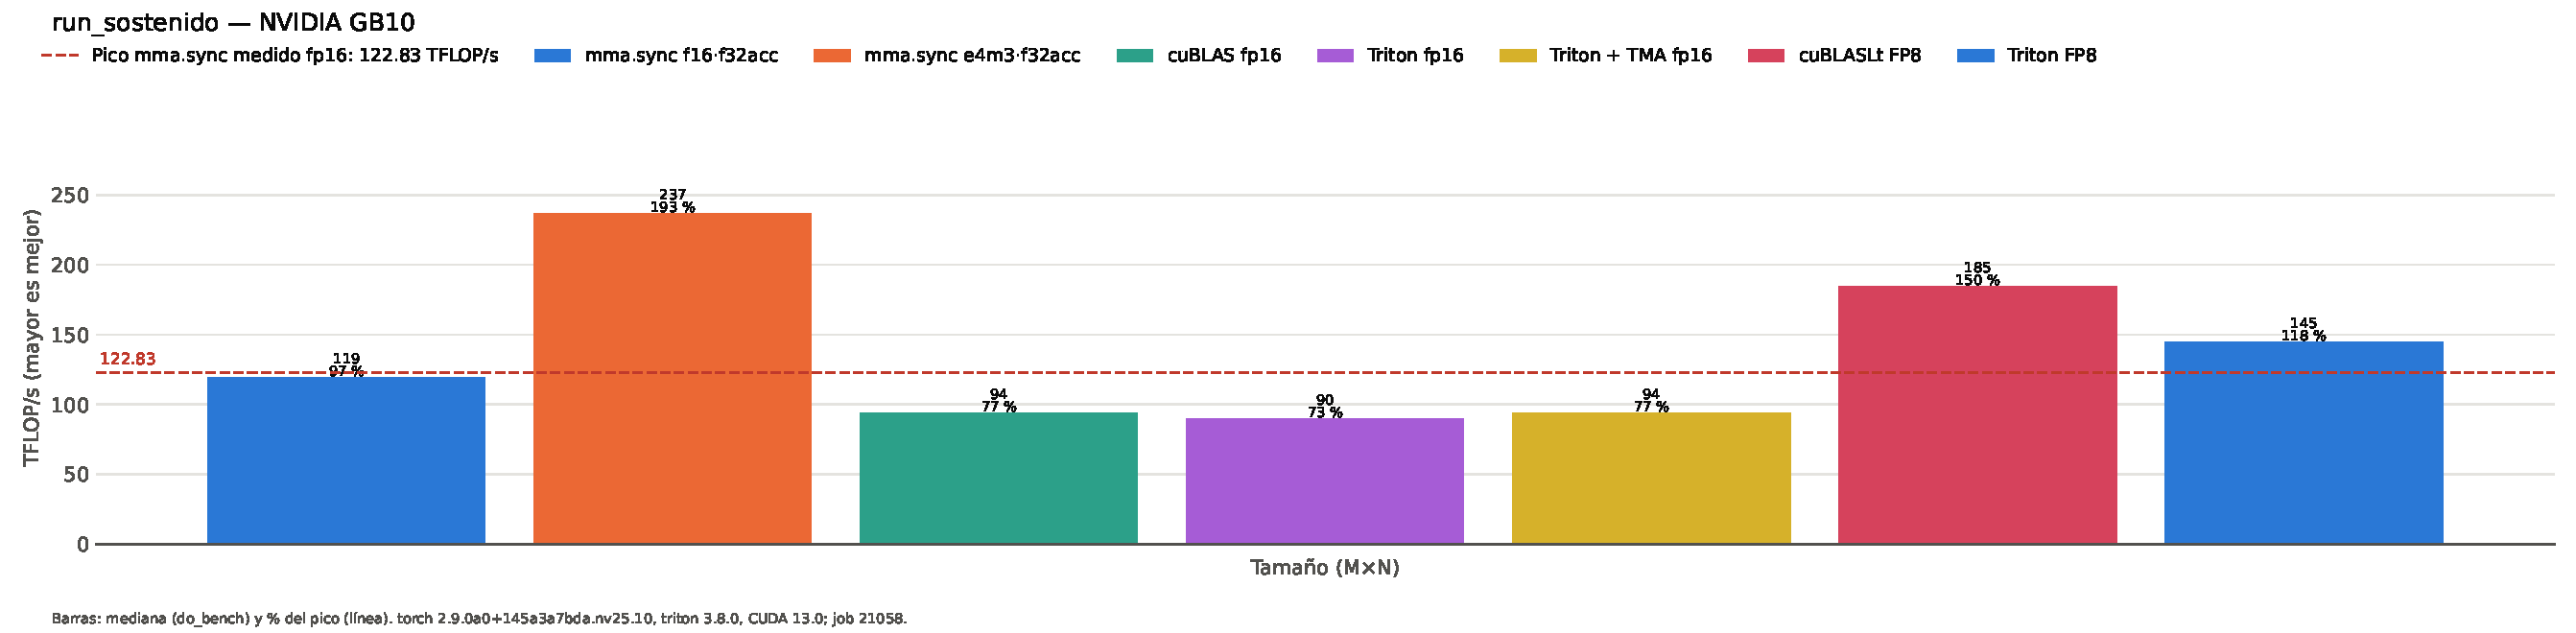
\includegraphics[width=\linewidth]{resultados/hennessy/figuras/run_sostenido.pdf}
  \caption{Régimen sostenido en GB10 (job 20848): (a) eficiencia por ciclo, como \% del pico de
  \texttt{mma.sync} al reloj de cada kernel; (b) reloj SM sostenido y potencia de GPU. La línea
  discontinua es el reloj que sostiene la MMA pura.}
  \label{fig:sostenido}
\end{figure}

En FlashAttention (jobs anteriores, sin reloj) los porcentajes sobre el pico nominal son: Triton
75\,\%, CuTe 74\,\% (normal y causal), SDPA 69\,\% y Helion 54\,\% (34\,\% causal, que además
no se salta el triángulo superior).

\begin{enumerate}
  \item \textbf{Ningún kernel real pasa del $\sim$77\,\% del pico nominal}, y el hueco tiene dos
  partes de tamaño parecido.
  \item \textbf{Reloj ($\sim$12--15 puntos).} La MMA pura sostiene 2\,424~MHz, pero cualquier
  GEMM real baja a 2\,080--2\,180~MHz, y lo hace con \emph{menos} potencia de GPU según NVML
  ($\sim$90 frente a 100~W). El límite no es, por tanto, la potencia de la GPU tal como la mide
  NVML. Una hipótesis plausible, pendiente de verificar, es el presupuesto total del chip, que
  comparte potencia y memoria con la CPU.
  \item \textbf{Por ciclo ($\sim$8--15 puntos).} A su propio reloj, cuBLAS y Triton + TMA llegan
  al 90--92\,\%. Lo que falta se pierde en alimentar \texttt{mma.sync} (\texttt{ldmatrix}, esperas
  de copia, sincronización, \emph{epilogue}).
  \item \textbf{TMA mejora la eficiencia por ciclo} (91{,}7 frente a 84{,}6\,\%), aunque su kernel
  sostiene un reloj algo menor. El neto es $+3{,}5\,\%$ (§~\ref{sec:tma}).
  \item \textbf{En FP8, Triton se queda en el 68\,\% a su reloj} (cuBLASLt, 87\,\%): hueco de
  \emph{scheduling} (§~\ref{sec:fp8}).
\end{enumerate}

\subsection{Conclusión}

La unidad MMA de GB10 hace \textbf{1\,024~FLOP/ciclo/SM en FP16/BF16, 2\,048 en FP8/INT8 y
4\,096 en MXFP4/NVFP4}, sin penalización por acumular en FP32 ni por el escalado por bloques: en
ráfaga, 122{,}7 / 243 / 487~TFLOP/s, y en régimen sostenido la MMA pura mantiene 2{,}42~GHz.
Saturarla requiere al menos dos warps por subpartición. Los mejores kernels del TFM sostienen el
75--77\,\% del pico nominal. Aproximadamente la mitad del hueco es reloj, porque un GEMM real
hace bajar GB10 a $\sim$2{,}1--2{,}2~GHz; la otra mitad se pierde por ciclo, alimentando la MMA.
A su propio reloj, estos kernels rinden el 87--92\,\% del pico. FP4 con escalado por bloques
duplica el techo de FP8 y es la palanca que queda por explotar.
.
% Requiere: \usepackage{graphicx,booktabs}. Ajusta rutas si compilas desde otro dir.
% Datos: results/hennessy/run_pico_mma/ultimo (job 20834) y matmul con reloj (jobs 20835--20837).
% GB10 (sm_121, 48 SMs), CUDA 13.0.

\section{Pico real de los tensor cores: microbenchmark de \texttt{mma.sync}}
\label{sec:pico-mma}

En Blackwell GeForce (sm\_120/sm\_121) no existen \texttt{wgmma} ni \texttt{tcgen05}, y todos
los DSLs acaban emitiendo \texttt{mma.sync} (§~\ref{sec:tma}). El techo de los kernels es, por
tanto, el ritmo de esa instrucción. NVIDIA no lo publica para sm\_121 y las cifras de catálogo
mezclan \emph{sparsity} y precisiones bajas, así que hasta ahora los kernels solo podían
compararse entre sí o con cuBLAS. Esta sección mide ese techo directamente, instrucción a
instrucción, y expresa los resultados del TFM como porcentaje del pico alcanzable.

\subsection{Método}

Un kernel CUDA con PTX en línea (\texttt{src/Microbench/pico\_mma\_ext.cu}) en el que cada warp
carga una sola vez sus fragmentos A y B en registros (datos aleatorios del tipo
correspondiente, no ceros, para no falsear la potencia). Después encadena
$\mathit{iters}\times\mathit{ILP}$ instrucciones \texttt{mma.sync} sobre ILP acumuladores
independientes, \textbf{sin ningún acceso a memoria}, y al final escribe un único valor por hilo
para que el compilador no elimine el bucle. Se lanza un bloque por SM y se barren los warps por
SM (1, 4, 8, 16, 32) y el ILP (1, 2, 4, 8). La medida es la mediana de \texttt{do\_bench}, y en
paralelo se muestrean el reloj SM y la potencia por NVML, de lo que se obtiene la cifra
intrínseca de la arquitectura: FLOP/ciclo/SM.

Cada instrucción se compila para \texttt{sm\_121a}, la variante específica de la arquitectura
y la única que acepta las MMA con escalado por bloques. Con \texttt{-arch=sm\_121a -shared},
nvcc genera PTX para \texttt{compute\_121} sin la \texttt{a} y ptxas las rechaza; hace falta
\texttt{-gencode=arch=compute\_121a,code=sm\_121a} explícito. El SASS (\texttt{cuobjdump})
confirma que todas se ejecutan como instrucciones de tensor core.

\subsection{Resultados}

\begin{figure}[htbp]
  \centering
  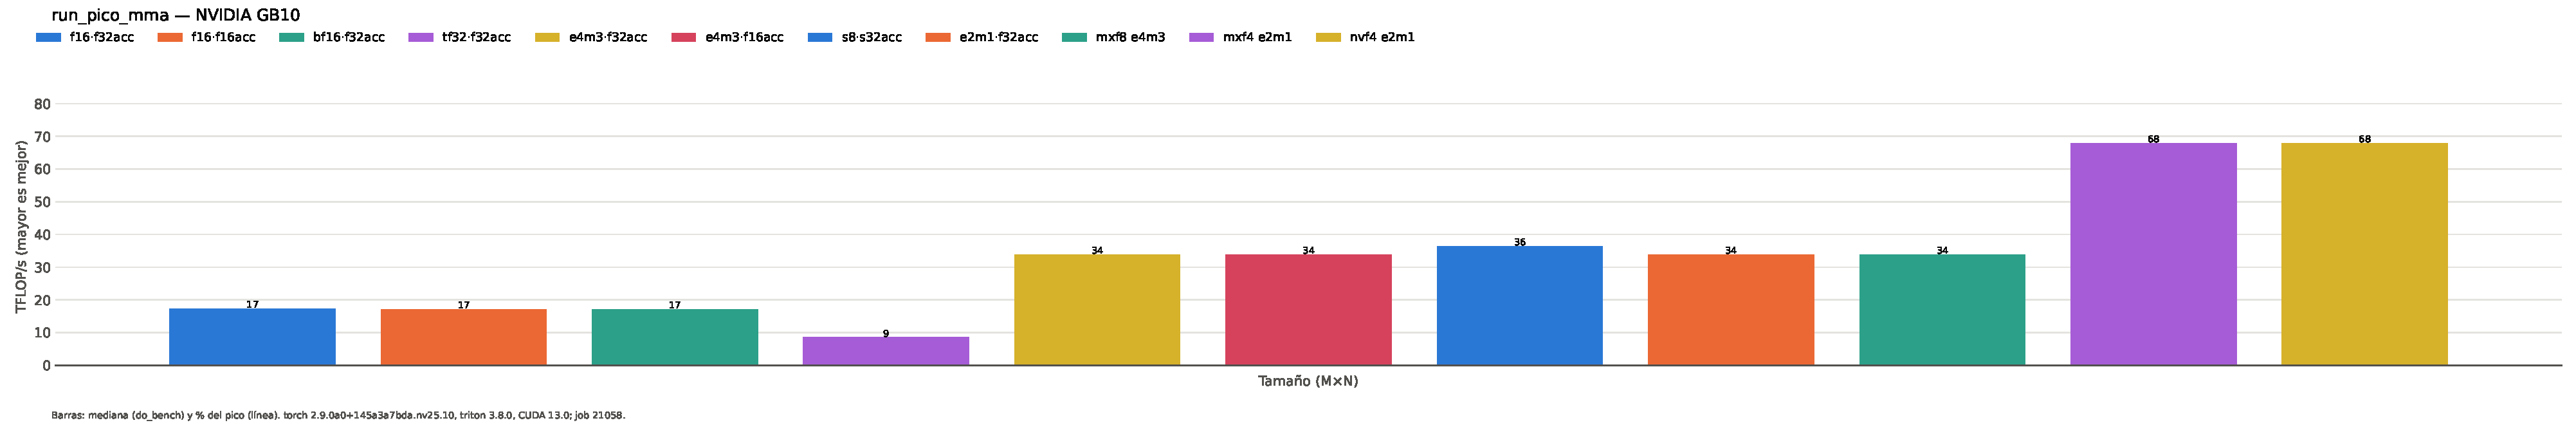
\includegraphics[width=\linewidth]{resultados/hennessy/figuras/run_pico_mma.pdf}
  \caption{GB10: (a) pico medido por instrucción \texttt{mma.sync}; (b) saturación de la
  unidad MMA (f16$\to$f32) en función de los warps por SM y de los acumuladores
  independientes por warp (ILP).}
  \label{fig:pico-mma}
\end{figure}

\begin{table}[htbp]
  \centering\small
  \begin{tabular}{llrrr}
    \toprule
    instrucción PTX & SASS & pico (TFLOP/s) & FLOP/ciclo/SM & rel.\ a f16 \\
    \midrule
    \texttt{m16n8k8} tf32$\to$f32 & \texttt{HMMA.1688.F32.TF32} & 61{,}4 & 511 & 0{,}5$\times$ \\
    \texttt{m16n8k16} f16$\to$f32 & \texttt{HMMA.16816.F32} & \textbf{122{,}7} & 1\,024 & 1$\times$ \\
    \texttt{m16n8k16} f16$\to$f16 & \texttt{HMMA.16816.F16} & 122{,}8 & 1\,020 & 1$\times$ \\
    \texttt{m16n8k16} bf16$\to$f32 & \texttt{HMMA.16816.F32.BF16} & 122{,}8 & 1\,019 & 1$\times$ \\
    \texttt{m16n8k32} e4m3$\to$f32 & \texttt{QMMA.16832.F32.E4M3} & \textbf{243{,}3} & 2\,041 & 2$\times$ \\
    \texttt{m16n8k32} e4m3$\to$f16 & \texttt{QMMA.16832.F16.E4M3} & 243{,}5 & 2\,038 & 2$\times$ \\
    \texttt{m16n8k32} s8$\to$s32 & \texttt{IMMA.16832.S8.S8} & 243{,}9\,(TOP/s) & 2\,031 & 2$\times$ \\
    \texttt{kind::f8f6f4} e2m1 & \texttt{QMMA.16832.F32.E2M1} & 245{,}7 & 2\,051 & 2$\times$ \\
    \texttt{kind::mxf8f6f4} MXFP8 & \texttt{QMMA.SF.16832.E4M3.E8} & 242{,}9 & 2\,038 & 2$\times$ \\
    \texttt{kind::mxf4nvf4} MXFP4 & \texttt{OMMA.SF.16864.E2M1.E8} & \textbf{487{,}3} & 4\,089 & 4$\times$ \\
    \texttt{kind::mxf4nvf4} NVFP4 & \texttt{OMMA.SF.16864.E2M1.UE4M3} & 486{,}9 & 4\,085 & 4$\times$ \\
    \bottomrule
  \end{tabular}
  \caption{Pico de \texttt{mma.sync} en GB10 (job 20834), en ráfaga ($\sim$0{,}35~s por punto,
  reloj 2\,480--2\,520~MHz). En régimen sostenido la MMA pura mantiene 2\,424~MHz: 118{,}7 (f16) y
  237{,}3 (e4m3) TFLOP/s (job 20848). Barrido completo en \texttt{resultados/hennessy/run\_pico\_mma}.}
  \label{tab:pico-mma}
\end{table}

\subsection{Análisis del microbenchmark}

\begin{enumerate}
  \item \textbf{La unidad MMA hace 1\,024~FLOP/ciclo/SM en FP16} (512 FMA, 128 por subpartición):
  122{,}7~TFLOP/s en ráfaga ($48~\text{SMs}\times 2{,}5~\text{GHz}$) y 118{,}7 sostenidos
  (2{,}42~GHz). La cifra por ciclo es la intrínseca; los TFLOP/s dependen del reloj sostenido.
  \item \textbf{Acumular en FP16 no aporta nada}: f16$\to$f16 rinde igual que f16$\to$f32 (lo
  mismo con e4m3). A diferencia de las GeForce Ampere/Ada, GB10 no reduce a la mitad la
  acumulación en FP32.
  \item \textbf{La escalera de precisiones es limpia}: TF32 0{,}5$\times$, FP16/BF16 1$\times$,
  FP8/INT8 2$\times$, FP4 4$\times$. Pero el 4$\times$ de FP4 solo se obtiene con la instrucción
  \emph{block-scaled} \texttt{mxf4nvf4} (\texttt{OMMA}, $k=64$, FP4 empaquetado). El FP4 de
  \texttt{kind::f8f6f4} usa contenedores de 8~bits y rinde como FP8. El escalado por bloques
  (MXFP8, MXFP4, NVFP4) no tiene coste.
  \item \textbf{Saturar la MMA exige $\geq 8$ warps por SM} ($\geq 2$ por subpartición). La
  latencia de una MMA es de $\sim$28 ciclos, y un mismo warp no emite más de una cada
  $\sim$17 ciclos, mientras que la unidad acepta una cada 16 por subpartición. Con 4~warps/SM el
  máximo es el $\sim$94\,\%, sea cual sea el ILP (figura~\ref{fig:pico-mma}b).
\end{enumerate}

\subsection{Medir reloj y potencia en GB10}

Como el pico es $1\,024~\text{FLOP/ciclo/SM}\times 48\times\text{reloj}$, comparar un kernel con él
exige saber a qué reloj iba. En GB10 eso no es trivial (sondas, jobs 20844 y 20845). NVML solo
actualiza reloj y potencia cada $\sim$0{,}5~s, y la potencia de \texttt{nvmlDeviceGetPowerUsage}
es un promedio retrasado $\sim$1~s: al empezar una carga, la potencia instantánea
(\texttt{NVML\_FI\_DEV\_POWER\_INSTANT}) ya marca 100~W y la promedio aún 20~W. Además, bajo un
GEMM continuo el reloj tarda $\sim$0{,}5~s en bajar de 2\,410 a 2\,180~MHz. Una medida de
\texttt{do\_bench} ($\sim$0{,}6~s) cae, por tanto, sobre el transitorio. Por eso se mide en
\textbf{régimen sostenido} (\texttt{run\_sostenido}): 6~s seguidos tras 3~s de reposo, contando
solo los últimos 4~s y con potencia instantánea. Una lectura previa con potencia promedio
(``TMA ahorra un tercio de potencia'') resultó ser un artefacto de la medida.

\subsection{Los kernels del TFM frente al pico}

\begin{table}[htbp]
  \centering\small
  \begin{tabular}{lrrrrr}
    \toprule
    kernel ($8192^3$) & TFLOP/s & reloj (MHz) & potencia (W) & \% al mismo reloj & \% nominal \\
    \midrule
    \texttt{mma.sync} f16 (micro) & 118{,}7 & 2\,424 & 100 & 99{,}6 & 97 \\
    \texttt{mma.sync} e4m3 (micro) & 237{,}3 & 2\,424 & 99 & 99{,}6 & 98 \\
    cuBLAS fp16 & 94{,}4 & 2\,138 & 90 & \textbf{89{,}8} & 77 \\
    Triton fp16 & 90{,}6 & 2\,177 & 90 & 84{,}6 & 74 \\
    Triton + TMA fp16 & 93{,}8 & 2\,080 & 89 & \textbf{91{,}7} & 76 \\
    cuBLASLt FP8 & 182{,}9 & 2\,145 & 91 & 86{,}7 & 75 \\
    Triton FP8 & 144{,}0 & 2\,158 & 91 & 67{,}9 & 59 \\
    \bottomrule
  \end{tabular}
  \caption{Régimen sostenido en GB10 (job 20848). ``Al mismo reloj'': frente a
  $1\,024$ (fp16) o $2\,048$ (fp8)~FLOP/ciclo/SM $\times$ 48 SMs al reloj medido durante el
  kernel. ``Nominal'': frente a 122{,}7 / 243{,}3~TFLOP/s (ráfaga a $\sim$2{,}5~GHz).}
  \label{tab:pico-kernels}
\end{table}

\begin{figure}[htbp]
  \centering
  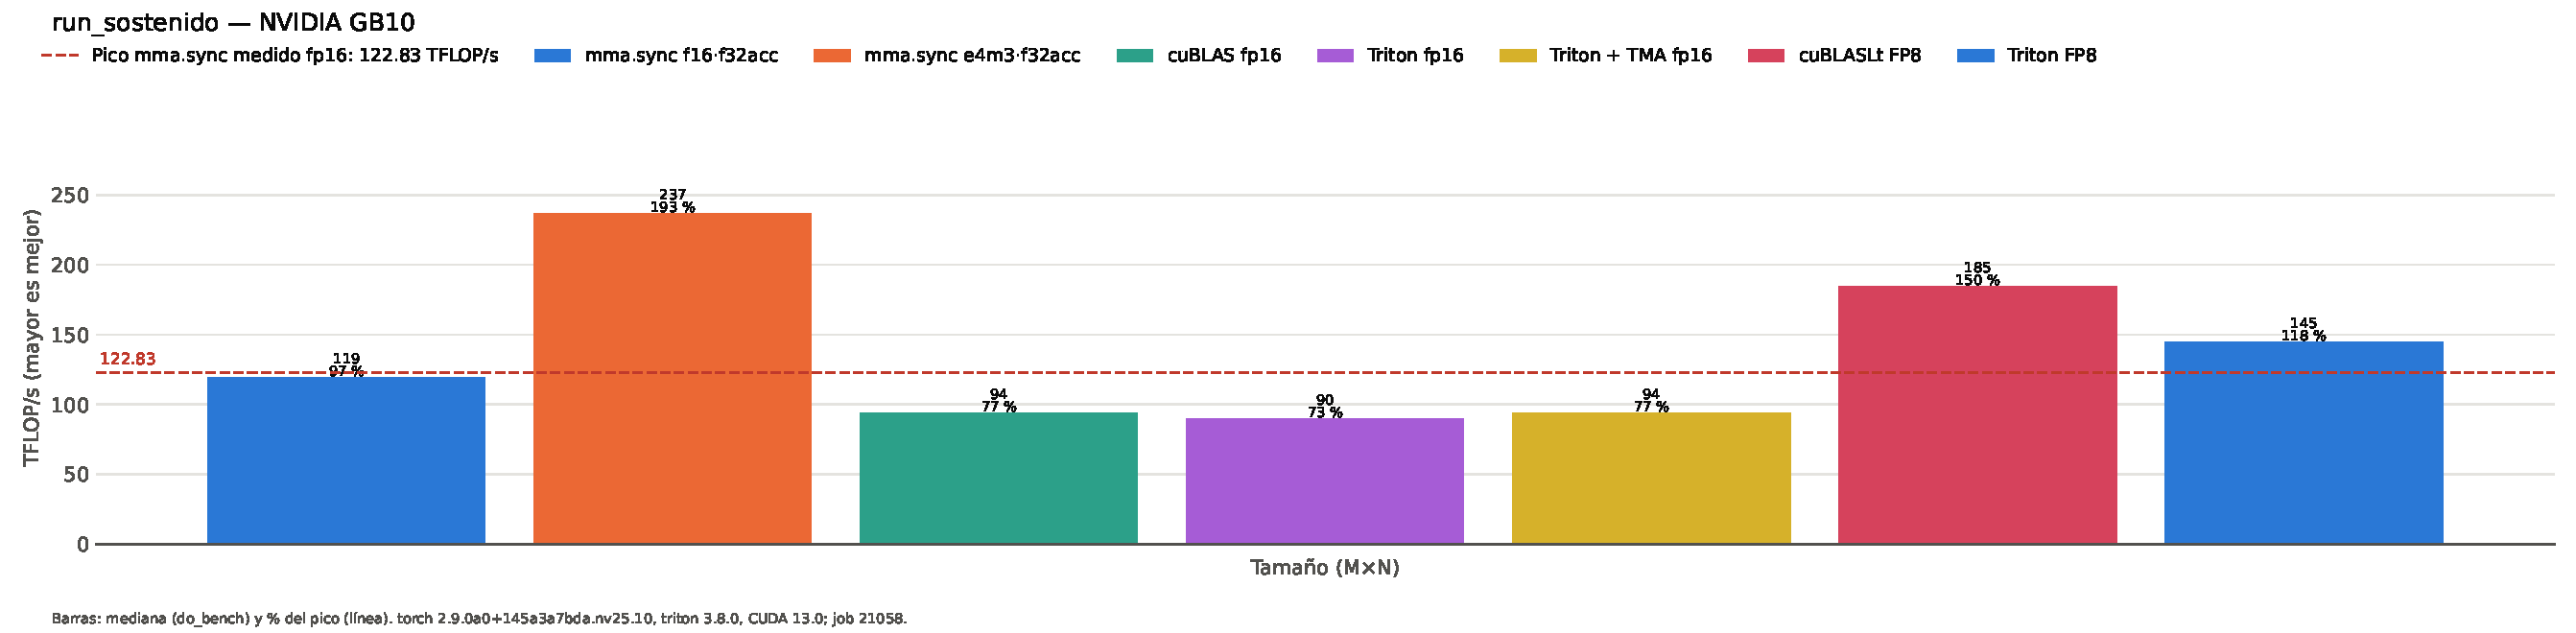
\includegraphics[width=\linewidth]{resultados/hennessy/figuras/run_sostenido.pdf}
  \caption{Régimen sostenido en GB10 (job 20848): (a) eficiencia por ciclo, como \% del pico de
  \texttt{mma.sync} al reloj de cada kernel; (b) reloj SM sostenido y potencia de GPU. La línea
  discontinua es el reloj que sostiene la MMA pura.}
  \label{fig:sostenido}
\end{figure}

En FlashAttention (jobs anteriores, sin reloj) los porcentajes sobre el pico nominal son: Triton
75\,\%, CuTe 74\,\% (normal y causal), SDPA 69\,\% y Helion 54\,\% (34\,\% causal, que además
no se salta el triángulo superior).

\begin{enumerate}
  \item \textbf{Ningún kernel real pasa del $\sim$77\,\% del pico nominal}, y el hueco tiene dos
  partes de tamaño parecido.
  \item \textbf{Reloj ($\sim$12--15 puntos).} La MMA pura sostiene 2\,424~MHz, pero cualquier
  GEMM real baja a 2\,080--2\,180~MHz, y lo hace con \emph{menos} potencia de GPU según NVML
  ($\sim$90 frente a 100~W). El límite no es, por tanto, la potencia de la GPU tal como la mide
  NVML. Una hipótesis plausible, pendiente de verificar, es el presupuesto total del chip, que
  comparte potencia y memoria con la CPU.
  \item \textbf{Por ciclo ($\sim$8--15 puntos).} A su propio reloj, cuBLAS y Triton + TMA llegan
  al 90--92\,\%. Lo que falta se pierde en alimentar \texttt{mma.sync} (\texttt{ldmatrix}, esperas
  de copia, sincronización, \emph{epilogue}).
  \item \textbf{TMA mejora la eficiencia por ciclo} (91{,}7 frente a 84{,}6\,\%), aunque su kernel
  sostiene un reloj algo menor. El neto es $+3{,}5\,\%$ (§~\ref{sec:tma}).
  \item \textbf{En FP8, Triton se queda en el 68\,\% a su reloj} (cuBLASLt, 87\,\%): hueco de
  \emph{scheduling} (§~\ref{sec:fp8}).
\end{enumerate}

\subsection{Conclusión}

La unidad MMA de GB10 hace \textbf{1\,024~FLOP/ciclo/SM en FP16/BF16, 2\,048 en FP8/INT8 y
4\,096 en MXFP4/NVFP4}, sin penalización por acumular en FP32 ni por el escalado por bloques: en
ráfaga, 122{,}7 / 243 / 487~TFLOP/s, y en régimen sostenido la MMA pura mantiene 2{,}42~GHz.
Saturarla requiere al menos dos warps por subpartición. Los mejores kernels del TFM sostienen el
75--77\,\% del pico nominal. Aproximadamente la mitad del hueco es reloj, porque un GEMM real
hace bajar GB10 a $\sim$2{,}1--2{,}2~GHz; la otra mitad se pierde por ciclo, alimentando la MMA.
A su propio reloj, estos kernels rinden el 87--92\,\% del pico. FP4 con escalado por bloques
duplica el techo de FP8 y es la palanca que queda por explotar.
.
% Requiere: \usepackage{graphicx,booktabs}. Ajusta rutas si compilas desde otro dir.
% Datos: results/hennessy/run_pico_mma/ultimo (job 20834) y matmul con reloj (jobs 20835--20837).
% GB10 (sm_121, 48 SMs), CUDA 13.0.

\section{Pico real de los tensor cores: microbenchmark de \texttt{mma.sync}}
\label{sec:pico-mma}

En Blackwell GeForce (sm\_120/sm\_121) no existen \texttt{wgmma} ni \texttt{tcgen05}, y todos
los DSLs acaban emitiendo \texttt{mma.sync} (§~\ref{sec:tma}). El techo de los kernels es, por
tanto, el ritmo de esa instrucción. NVIDIA no lo publica para sm\_121 y las cifras de catálogo
mezclan \emph{sparsity} y precisiones bajas, así que hasta ahora los kernels solo podían
compararse entre sí o con cuBLAS. Esta sección mide ese techo directamente, instrucción a
instrucción, y expresa los resultados del TFM como porcentaje del pico alcanzable.

\subsection{Método}

Un kernel CUDA con PTX en línea (\texttt{src/Microbench/pico\_mma\_ext.cu}) en el que cada warp
carga una sola vez sus fragmentos A y B en registros (datos aleatorios del tipo
correspondiente, no ceros, para no falsear la potencia). Después encadena
$\mathit{iters}\times\mathit{ILP}$ instrucciones \texttt{mma.sync} sobre ILP acumuladores
independientes, \textbf{sin ningún acceso a memoria}, y al final escribe un único valor por hilo
para que el compilador no elimine el bucle. Se lanza un bloque por SM y se barren los warps por
SM (1, 4, 8, 16, 32) y el ILP (1, 2, 4, 8). La medida es la mediana de \texttt{do\_bench}, y en
paralelo se muestrean el reloj SM y la potencia por NVML, de lo que se obtiene la cifra
intrínseca de la arquitectura: FLOP/ciclo/SM.

Cada instrucción se compila para \texttt{sm\_121a}, la variante específica de la arquitectura
y la única que acepta las MMA con escalado por bloques. Con \texttt{-arch=sm\_121a -shared},
nvcc genera PTX para \texttt{compute\_121} sin la \texttt{a} y ptxas las rechaza; hace falta
\texttt{-gencode=arch=compute\_121a,code=sm\_121a} explícito. El SASS (\texttt{cuobjdump})
confirma que todas se ejecutan como instrucciones de tensor core.

\subsection{Resultados}

\begin{figure}[htbp]
  \centering
  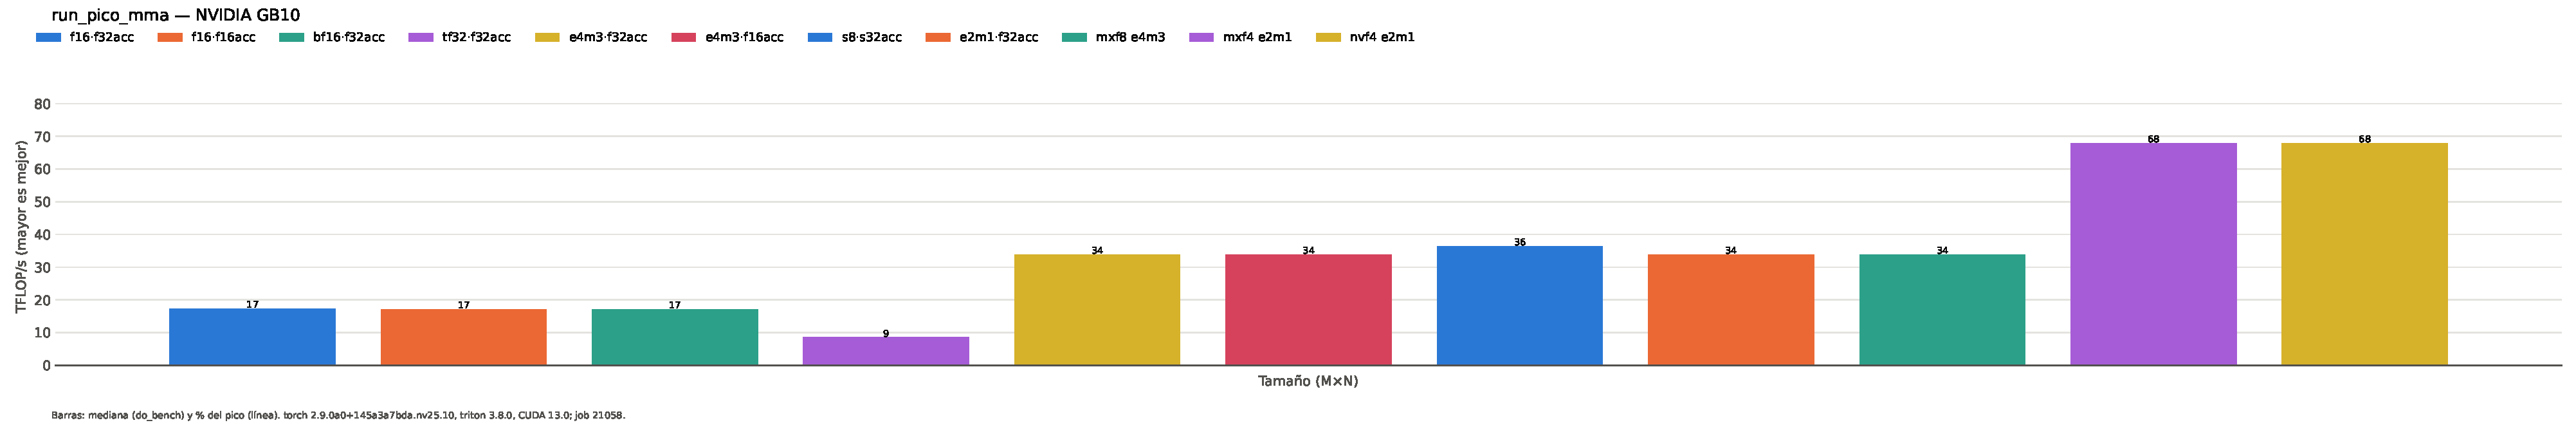
\includegraphics[width=\linewidth]{resultados/hennessy/figuras/run_pico_mma.pdf}
  \caption{GB10: (a) pico medido por instrucción \texttt{mma.sync}; (b) saturación de la
  unidad MMA (f16$\to$f32) en función de los warps por SM y de los acumuladores
  independientes por warp (ILP).}
  \label{fig:pico-mma}
\end{figure}

\begin{table}[htbp]
  \centering\small
  \begin{tabular}{llrrr}
    \toprule
    instrucción PTX & SASS & pico (TFLOP/s) & FLOP/ciclo/SM & rel.\ a f16 \\
    \midrule
    \texttt{m16n8k8} tf32$\to$f32 & \texttt{HMMA.1688.F32.TF32} & 61{,}4 & 511 & 0{,}5$\times$ \\
    \texttt{m16n8k16} f16$\to$f32 & \texttt{HMMA.16816.F32} & \textbf{122{,}7} & 1\,024 & 1$\times$ \\
    \texttt{m16n8k16} f16$\to$f16 & \texttt{HMMA.16816.F16} & 122{,}8 & 1\,020 & 1$\times$ \\
    \texttt{m16n8k16} bf16$\to$f32 & \texttt{HMMA.16816.F32.BF16} & 122{,}8 & 1\,019 & 1$\times$ \\
    \texttt{m16n8k32} e4m3$\to$f32 & \texttt{QMMA.16832.F32.E4M3} & \textbf{243{,}3} & 2\,041 & 2$\times$ \\
    \texttt{m16n8k32} e4m3$\to$f16 & \texttt{QMMA.16832.F16.E4M3} & 243{,}5 & 2\,038 & 2$\times$ \\
    \texttt{m16n8k32} s8$\to$s32 & \texttt{IMMA.16832.S8.S8} & 243{,}9\,(TOP/s) & 2\,031 & 2$\times$ \\
    \texttt{kind::f8f6f4} e2m1 & \texttt{QMMA.16832.F32.E2M1} & 245{,}7 & 2\,051 & 2$\times$ \\
    \texttt{kind::mxf8f6f4} MXFP8 & \texttt{QMMA.SF.16832.E4M3.E8} & 242{,}9 & 2\,038 & 2$\times$ \\
    \texttt{kind::mxf4nvf4} MXFP4 & \texttt{OMMA.SF.16864.E2M1.E8} & \textbf{487{,}3} & 4\,089 & 4$\times$ \\
    \texttt{kind::mxf4nvf4} NVFP4 & \texttt{OMMA.SF.16864.E2M1.UE4M3} & 486{,}9 & 4\,085 & 4$\times$ \\
    \bottomrule
  \end{tabular}
  \caption{Pico de \texttt{mma.sync} en GB10 (job 20834), en ráfaga ($\sim$0{,}35~s por punto,
  reloj 2\,480--2\,520~MHz). En régimen sostenido la MMA pura mantiene 2\,424~MHz: 118{,}7 (f16) y
  237{,}3 (e4m3) TFLOP/s (job 20848). Barrido completo en \texttt{resultados/hennessy/run\_pico\_mma}.}
  \label{tab:pico-mma}
\end{table}

\subsection{Análisis del microbenchmark}

\begin{enumerate}
  \item \textbf{La unidad MMA hace 1\,024~FLOP/ciclo/SM en FP16} (512 FMA, 128 por subpartición):
  122{,}7~TFLOP/s en ráfaga ($48~\text{SMs}\times 2{,}5~\text{GHz}$) y 118{,}7 sostenidos
  (2{,}42~GHz). La cifra por ciclo es la intrínseca; los TFLOP/s dependen del reloj sostenido.
  \item \textbf{Acumular en FP16 no aporta nada}: f16$\to$f16 rinde igual que f16$\to$f32 (lo
  mismo con e4m3). A diferencia de las GeForce Ampere/Ada, GB10 no reduce a la mitad la
  acumulación en FP32.
  \item \textbf{La escalera de precisiones es limpia}: TF32 0{,}5$\times$, FP16/BF16 1$\times$,
  FP8/INT8 2$\times$, FP4 4$\times$. Pero el 4$\times$ de FP4 solo se obtiene con la instrucción
  \emph{block-scaled} \texttt{mxf4nvf4} (\texttt{OMMA}, $k=64$, FP4 empaquetado). El FP4 de
  \texttt{kind::f8f6f4} usa contenedores de 8~bits y rinde como FP8. El escalado por bloques
  (MXFP8, MXFP4, NVFP4) no tiene coste.
  \item \textbf{Saturar la MMA exige $\geq 8$ warps por SM} ($\geq 2$ por subpartición). La
  latencia de una MMA es de $\sim$28 ciclos, y un mismo warp no emite más de una cada
  $\sim$17 ciclos, mientras que la unidad acepta una cada 16 por subpartición. Con 4~warps/SM el
  máximo es el $\sim$94\,\%, sea cual sea el ILP (figura~\ref{fig:pico-mma}b).
\end{enumerate}

\subsection{Medir reloj y potencia en GB10}

Como el pico es $1\,024~\text{FLOP/ciclo/SM}\times 48\times\text{reloj}$, comparar un kernel con él
exige saber a qué reloj iba. En GB10 eso no es trivial (sondas, jobs 20844 y 20845). NVML solo
actualiza reloj y potencia cada $\sim$0{,}5~s, y la potencia de \texttt{nvmlDeviceGetPowerUsage}
es un promedio retrasado $\sim$1~s: al empezar una carga, la potencia instantánea
(\texttt{NVML\_FI\_DEV\_POWER\_INSTANT}) ya marca 100~W y la promedio aún 20~W. Además, bajo un
GEMM continuo el reloj tarda $\sim$0{,}5~s en bajar de 2\,410 a 2\,180~MHz. Una medida de
\texttt{do\_bench} ($\sim$0{,}6~s) cae, por tanto, sobre el transitorio. Por eso se mide en
\textbf{régimen sostenido} (\texttt{run\_sostenido}): 6~s seguidos tras 3~s de reposo, contando
solo los últimos 4~s y con potencia instantánea. Una lectura previa con potencia promedio
(``TMA ahorra un tercio de potencia'') resultó ser un artefacto de la medida.

\subsection{Los kernels del TFM frente al pico}

\begin{table}[htbp]
  \centering\small
  \begin{tabular}{lrrrrr}
    \toprule
    kernel ($8192^3$) & TFLOP/s & reloj (MHz) & potencia (W) & \% al mismo reloj & \% nominal \\
    \midrule
    \texttt{mma.sync} f16 (micro) & 118{,}7 & 2\,424 & 100 & 99{,}6 & 97 \\
    \texttt{mma.sync} e4m3 (micro) & 237{,}3 & 2\,424 & 99 & 99{,}6 & 98 \\
    cuBLAS fp16 & 94{,}4 & 2\,138 & 90 & \textbf{89{,}8} & 77 \\
    Triton fp16 & 90{,}6 & 2\,177 & 90 & 84{,}6 & 74 \\
    Triton + TMA fp16 & 93{,}8 & 2\,080 & 89 & \textbf{91{,}7} & 76 \\
    cuBLASLt FP8 & 182{,}9 & 2\,145 & 91 & 86{,}7 & 75 \\
    Triton FP8 & 144{,}0 & 2\,158 & 91 & 67{,}9 & 59 \\
    \bottomrule
  \end{tabular}
  \caption{Régimen sostenido en GB10 (job 20848). ``Al mismo reloj'': frente a
  $1\,024$ (fp16) o $2\,048$ (fp8)~FLOP/ciclo/SM $\times$ 48 SMs al reloj medido durante el
  kernel. ``Nominal'': frente a 122{,}7 / 243{,}3~TFLOP/s (ráfaga a $\sim$2{,}5~GHz).}
  \label{tab:pico-kernels}
\end{table}

\begin{figure}[htbp]
  \centering
  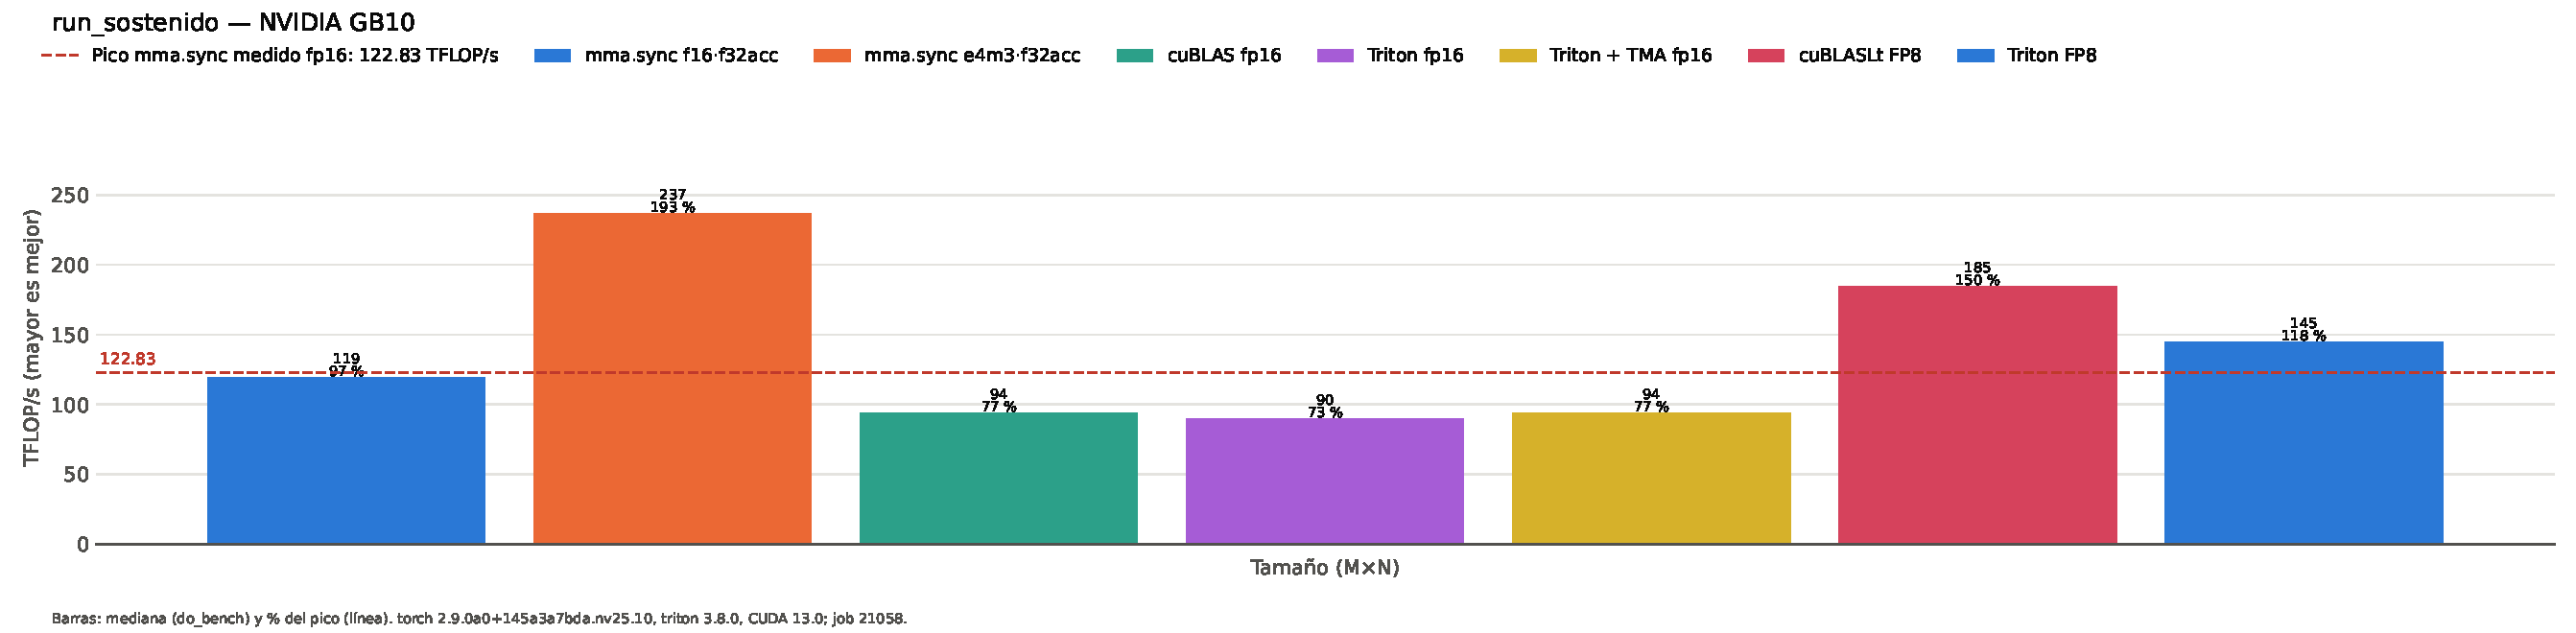
\includegraphics[width=\linewidth]{resultados/hennessy/figuras/run_sostenido.pdf}
  \caption{Régimen sostenido en GB10 (job 20848): (a) eficiencia por ciclo, como \% del pico de
  \texttt{mma.sync} al reloj de cada kernel; (b) reloj SM sostenido y potencia de GPU. La línea
  discontinua es el reloj que sostiene la MMA pura.}
  \label{fig:sostenido}
\end{figure}

En FlashAttention (jobs anteriores, sin reloj) los porcentajes sobre el pico nominal son: Triton
75\,\%, CuTe 74\,\% (normal y causal), SDPA 69\,\% y Helion 54\,\% (34\,\% causal, que además
no se salta el triángulo superior).

\begin{enumerate}
  \item \textbf{Ningún kernel real pasa del $\sim$77\,\% del pico nominal}, y el hueco tiene dos
  partes de tamaño parecido.
  \item \textbf{Reloj ($\sim$12--15 puntos).} La MMA pura sostiene 2\,424~MHz, pero cualquier
  GEMM real baja a 2\,080--2\,180~MHz, y lo hace con \emph{menos} potencia de GPU según NVML
  ($\sim$90 frente a 100~W). El límite no es, por tanto, la potencia de la GPU tal como la mide
  NVML. Una hipótesis plausible, pendiente de verificar, es el presupuesto total del chip, que
  comparte potencia y memoria con la CPU.
  \item \textbf{Por ciclo ($\sim$8--15 puntos).} A su propio reloj, cuBLAS y Triton + TMA llegan
  al 90--92\,\%. Lo que falta se pierde en alimentar \texttt{mma.sync} (\texttt{ldmatrix}, esperas
  de copia, sincronización, \emph{epilogue}).
  \item \textbf{TMA mejora la eficiencia por ciclo} (91{,}7 frente a 84{,}6\,\%), aunque su kernel
  sostiene un reloj algo menor. El neto es $+3{,}5\,\%$ (§~\ref{sec:tma}).
  \item \textbf{En FP8, Triton se queda en el 68\,\% a su reloj} (cuBLASLt, 87\,\%): hueco de
  \emph{scheduling} (§~\ref{sec:fp8}).
\end{enumerate}

\subsection{Conclusión}

La unidad MMA de GB10 hace \textbf{1\,024~FLOP/ciclo/SM en FP16/BF16, 2\,048 en FP8/INT8 y
4\,096 en MXFP4/NVFP4}, sin penalización por acumular en FP32 ni por el escalado por bloques: en
ráfaga, 122{,}7 / 243 / 487~TFLOP/s, y en régimen sostenido la MMA pura mantiene 2{,}42~GHz.
Saturarla requiere al menos dos warps por subpartición. Los mejores kernels del TFM sostienen el
75--77\,\% del pico nominal. Aproximadamente la mitad del hueco es reloj, porque un GEMM real
hace bajar GB10 a $\sim$2{,}1--2{,}2~GHz; la otra mitad se pierde por ciclo, alimentando la MMA.
A su propio reloj, estos kernels rinden el 87--92\,\% del pico. FP4 con escalado por bloques
duplica el techo de FP8 y es la palanca que queda por explotar.
